\documentclass[12pt,a4paper]{article}
\usepackage[utf8]{inputenc}
\usepackage[T1]{fontenc}
\usepackage[ngerman]{babel}
\usepackage{amsmath}
\usepackage{amsfonts}
\usepackage{amssymb}
\usepackage{lmodern}
\usepackage{tikz-uml}
\usepackage[singlelinecheck=off, list=off]{caption}
\usepackage{enumitem}
\usepackage[backend=bibtex]{biblatex} 
\makeatletter
\def\blx@maxline{77}
\makeatother
\addbibresource{literatur.bib}
\usepackage[colorlinks]{hyperref}

\newcommand*{\Title}{Projektseminar: Gestensteuerung einer 3D-Anwendung mittels Kinect}
\newcommand{\Authors}{Mario Janke,\\Peter Lindner,\\Patrick Stäblein}
\title{\Title}
\author{
	Mario Janke\\
	Peter Lindner\\
	Patrick Stäblein}
\date{}

\usepackage{fancyhdr}
\usepackage{vmargin}
\usepackage{setspace}
\onehalfspacing
\pagestyle{fancy}  %lustige fuß- und kopfzeilen
\parindent 0pt	
\parskip 0pt %
\emergencystretch 20pt
\setmarginsrb{3.0cm}{2.5cm}{2.5cm}{1.5cm}%  %ränder links oben rechts unten
             {1.0cm}{1.5cm}{1.0cm}{1.7cm}%  %kopf und fußzeile, höhe, abstand
\setlength{\leftmargin}{3.0cm}
\setlength{\textwidth}{15.5cm}
\setlength{\headwidth}{15.5cm}
\setlength{\topmargin}{2.0cm}
\lfoot{\footnotesize{\emph{\Title}}}
\cfoot{}
\rfoot{\footnotesize{\emph{\thepage}}}
\rhead{\emph{\leftmark}}
\chead{}
\lhead{}
\renewcommand{\footrulewidth}{0.5pt}
\renewcommand{\headrulewidth}{0.5pt}

\begin{document}
\maketitle
\tableofcontents
\clearpage
\section{Rahmenbedingungen}
	\subsection{Grundlagen und Motivation}
	Gegeben ist eine bereits vorhandene 3D-Anwendung, die vom Betreuer des Projektseminars, Herrn M.\,sc. Julian Meder, erstellt wurde. Das Programm wird zu Demonstrationszwecken z.\,B. am Tag der offenen Tür in den Räumlichkeiten des Fachgebiets genutzt. Innerhalb der Anwendung ist es möglich,
	\begin{itemize}
		\item Objekte einzuladen und anzeigen zu lassen sowie
		\item die Kamera (bzw. Kameras) zu manipulieren, d.\,h. zu bewegen, zu rotieren und zu zoomen.
	\end{itemize}
	In Erweiterung soll das Programm auch weiteren Aufgaben der Objektmanipulation dienlich sein, dies beinhaltet insbesondere das Laden mehrerer Objekte in eine Szene und die Manipulation dieser im Sinne von Translation, Rotation, Skalierung und Löschung.\par
	Den oben genannten Demonstrationszweck nimmt das Programm über die Ankopplung des Rechners an einen 3D-Kameraaufbau wahr. Das Programm rendert zwei Ausgabefenster aus zwei verschiedenen, im Sinne der Stereoskopie angeordneten Kamerasichten. Dies wird von den beiden Projektoren im Nebenraum des Päsentationsraums genutzt um ein linkes und ein rechtes Bild von hinten auf einen Schirm zu strahlen, der in die Trennwand der beiden Räume eingelassen ist. Mittels handelüblicher aus 3D-Kinos bekannten Shutterbrillen können Benutzer und Zuschauer sodann den 3D-Eindruck wahrnehmen.\par
	Die Steuerung des genannten Grundprogramms erfolgt durch den Vortragenden (im Weiteren zumeist Master genannt) über Tastatur und Maus bzw. einen Präsentationspointer. Die Unhandlichkeit sowie fehlende Immersion und Attraktivität dieser Steuerung ist eine Kernmotivation für unser Projekt. Darüber hinaus motivierend ist auch die bloße Auseinandersetzung mit der am Fachgebiet vorhandenen Technik sowie die Untersuchung der Möglichkeiten, diese zielführend einzusetzen.
	\subsection{Eigenschaften der Kinect} 
	Wir stellen in diesem Abschnitt nur die für uns interessanten Eigenschaften und Möglichkeiten der Kinect vor (hinsichtlich unserer Aufgabe und der Rahmenbedingungen). Die Kinect erkennt visuell den 3D-Raum vor sich. Dabei werden Personen als solche detektiert und konfidenzbasiert mit einem primitiven und grobgranularen Skelett ausgestattet. Dieses Tracking ist für bis zu sechs Personen zeitgleich möglich. Weiterhin wird für beide Hände einer getrackten Person ein \glqq Handzustand\grqq~erkannt, nämlich ob die Hand offen oder geschlossen ist, oder die sogenannte Lassogeste gebildet wird (etwa nur zwei Finger ausgestreckt). Kann einer Hand keiner dieser Zustände zugeordnet werden, ist ihr Status unbekannt. Diese Daten (Skelett und Status pro getrackter Person) können unter Verwendung der USB-Schnittstelle und des Kinect-SDKs abgegriffen werden. Sie werden dafür 30 mal in der Sekunde zur Verfügung gestellt.
	%
	%
\clearpage
\section{Vorüberlegungen}
	Für unser Vorgehen zentral sind die folgenden beiden Bereiche:
	\begin{enumerate}
		\item die technische Umsetzung, d.\,h.
		\begin{itemize}
		\item das korrekte Erkennen und Werten von Gesten einer ausgezeichneten getrackten Person
		\item das korrekte Berechnen notwendiger Bewegungsparameter
		\item die Einbindung in die bestehende Applikation
		\end{itemize}
		\item die Interaktion mit dem Benutzer, d.\,h.
		\begin{itemize}
		\item das Entwerfen intuitiver und eingängiger Gesten für die verschiedenen Zwecke
		\item das Auszeichnen einer getrackten Person als \glqq Master\grqq, der das Programm steuert
		\end{itemize}
	\end{enumerate}
	Wir stellen in diesem Abschnitt die zentralen unmittelbaren Beobachtungen vor, die sich aus der Aufgabenstellung und dem Versuchsaufbau ziehen lassen.\par\bigskip
	Ausgehend von der Aufgabenstellung kann man abstrahierend zwischen zwei primitiven Steuerungsmodi unterscheiden:
	\begin{itemize}
	\item einem Modus, in dem die Kamera verschoben und rotiert werden kann \&
	\item einem Modus, in welchem Objektmanipulationen möglich sind.
	\end{itemize}
	Der Benutzer sollte sich zu jedem Zeitpunkt nur in maximal einem dieser Modi aufhalten, d.\,h. gleichzeitige Kamera- und Objektmanipulation wird ausgeschlossen. Diese Vereinfachung treffen wir, da damit weniger komplexe Gesten benötigt werden und eine solche simultane Manipulation keine praktische Relevanz besitzt. Für Manipulationen, die man sowohl für die Kamera, als auch für Objekte haben will, bietet dies zudem eine geeignete Kapselung, da z.\,B. Rotationsparameter berechnet werden und dann nur entschieden werden muss, ob sie auf die Kamera oder ein Objekt angewendet werden, je nach Modus. Dies reduziert die Gesamtzahl nötiger Gesten.\par\medskip
	Die Kinect ermöglicht ein Tracking des gesamten Körpers für mehrere (genauer sechs) Personen. Wir beschränken uns aus naheliegenden Gründen jedoch auf einen Teil dieses Spektrums:
	\begin{itemize}
		\item Wir benötigen nur eine Person, die die Anwendung (möglichst ungestört) steuert. Eine genauere Auswertung der restlichen Personen, ihrer Skelette etc. ist unnötig.
		\item Die in unserem Anwendungsfall intuitiven Gesten werden ausschließlich mit den Händen (bzw. Armen) durchgeführt.
	\end{itemize}
	Primitive Erkennungsmöglichkeiten eines Masters kann man etwa aus der Entfernung der getrackten Personen zur Kamera und der Position der Personen im Raum gewinnen. Genauere Erklärungen folgen weiter unten.\par 
	Intuitive Gesten für Verschiebungen imitieren das Verschieben eines großen Gegenstands, etwa einer imaginären Box, sodass hier etwa ein Verschieben der flachen Hand in der Luft naheliegt. Für eine intuitive Drehgeste eignet sich die Vorstellung eines imaginären Lenkrads, genauer gesagt einer Lenkkugel, bei der die Rotation um eine Raumachse nach dem Lenkradprinzip erfolgt. Eine intuitive Geste zur Objektauswahl ist offenbar eine Greifgeste.
	\subsection{Priorisierung der Aufgaben}
	%TODO
	\subsection{Aufgabenverteilung im Team}
	%TODO
	Grob:
		Mario -- Algorithmik und Berechnung;
		Peter -- Backend, Struktur;
		Patrick -- Master, Kinect-Basics;
	Anmerkung, dass wir zu viert angefangen haben.
	%
	%
\clearpage
\section{Entwurfsentscheidungen}
	\subsection{Der Master}
	Der Master ist die Person (unter den getrackten Personen), der es obliegt, die Anwendung zu steuern, d.\,h. in unserem Anwendungsfall der Präsentation ist der Master der Präsentierende.\par
	Es muss gewährleistet werden, dass nur der Master das Programm steuert und dabei von weiteren Personen im Raum nicht (bzw. nicht ohne weiteres) gestört werden kann. Die Erkennung muss robust gegen Jittering der Kinectdaten sein.
	\subsection{Gesten und ihre Wirkung}
	Für die eingangs erwähnte Aufgabenstellung war es notwendig, bestimmte Programmfunktionalitäten mit Gesten zu verbinden. Einerseits hätte die Möglichkeit bestanden, mit dem Kinect-eigenen Visual Gesture Builder Gesten aufzunehmen und einzulernen. Diese Gesten werden dann als Datenbank ins Programm geladen und bei Vorführung erkannt. Dies erspart natürlich primitive aber umständliche Low-Level-Erkennungsmechanismen. Weiterhin sind hierdurch einige weiterführende Möglichkeiten gegeben wie etwa die Rückgabe, bis zu welchem Punkt eine Geste bereits ausgeführt wurde (in Bezug zur Gesamtgeste, d.\,h. beispielsweise wieviel Prozent einer Armbewegung vordefinierte Länge bereits ausgeführt wurde). Anderseits wiederum können durch die Kinect-Rohdaten auch eigene Erkennmechanismen implementiert werden. Dies bietet dem Programmierer die vollständige Kontrolle über seinen Gestenkatalog. Änderungen können kurzfristig und schnell vorgenommen werden und für einfache Projekte ist die Zusatzfunktionalität, die der Visual Gesture Builder gestattet nicht vonnöten, der eher für komplexere Gestenfolgen ausgelegt zu sein scheint. Demgegenüber ist für diese Direktimplementierung von Gesten aber die bereits erwähnte Low-Level-Erkennung zu implementieren, d.\,h. ein Extrahieren von Bewegungen und Bewegungsrichtungen aus den Skelett- und Gelenkdaten, die die Kinect bestimmt. Dennoch entschieden wir schließlich uns kraft dieser Gegenüberstellung (nebst einigen Versuchen mit dem Visual Gesture Builder, die uns nicht von seinem Mehrwert in unserer konkreten Anwendungssituation überzeugen konnten) für eine direkte Gestenerkennung.\par 
	Auch bei der Low-Level-Erkennung gibt es jedoch verschiedene Ansätze bzw. Ausprägungen. Es ist sogar das Implementieren nicht ganz primitiver Gestenfolgen möglich, indem eine Geste zeitlich und räumlich in verschiedene Segmente unterteilt wird. Dies sei an einem Beispiel erläutert: Es soll eine Winkgeste der rechten Hand erkannt werden. Die Geste wird in zwei Segmente geteilt. Ein Wechsel zwischen den Segmenten findet statt, wenn die horizontale Position der Hand und des Ellenbogens wechseln. Wird dieser Übergang dreimal in Folge erkannt, so wurde die Winkgeste präsentiert.\par
	Eine genauere Auseinandersetzung mit der Aufgabenstellung und unseren Vorstellungen von intuitiven Gesten für die zu realisierenden Funktionalitäten zeigte jedoch auf, dass auch eine Segmenteinteilung von Gesten für das Projekt nicht notwendig ist. Stattdessen sind die gegebenen Aufgaben in ihrer Struktur simpel genug, um die verschiedenen Wirkungen mit diskreten Gesten zu erzeugen, d.\,h. es genügt die Erkennung einer Geste durch bestimmte Zustände der Kinect-Rohdaten zu einem einzigen Zeitpunkt. Um die Wirkung jedoch zu erzielen, ist natürlich auch eine Betrachtung der Geste über mehrere Frames notwendig.\par\medskip
	Im Folgenden erklären wir unseren Gestenkatalog und gehen dabei darauf ein, was der Benutzer vorführen muss, damit die Geste erkannt wird und wie die Geste genutzt wird, um in der Anwendung die Kamera oder Objekte zu manipulieren:\par\bigskip
	\begin{description}
		\item[TRANSLATE\_GESTURE] (siehe Abb. \ref{fig:translateg})\par
		Der Benutzer hat beide Hände geöffnet, mit den Handflächen zur Kamera (wichtig ist nur, dass die Kinect beide Hände als offen erkennt, die genaue Haltung ist dabei egal). Ein paralleles Verschieben der beiden Hände in eine Richtung bewirkt ein zur Bewegungsgeschwindigkeit proportionales Verschieben der Kamera in diese Richtung.\par 
		Diese Geste war allen Projektteilnehmern unmittelbar einleuchtend und intuitiv und bedurfte keiner weiteren Diskussionen. 
		\begin{figure}[h!]
		\centering
		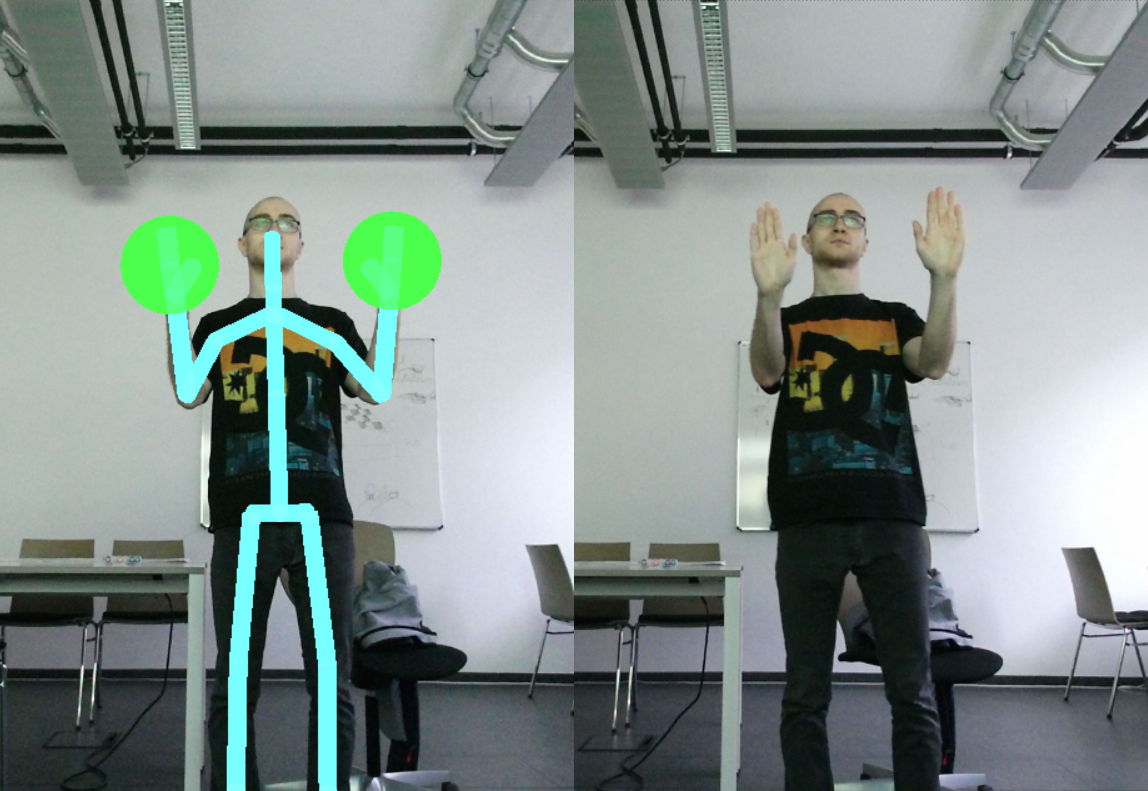
\includegraphics[width=.8\textwidth]{pictures/translate_.png}
		\caption{Die (Kamera-)Translations-Geste, mit und ohne eingezeichnetes Skelett und HandStates.}\label{fig:translateg}
		\end{figure}
		\par
		\item[ROTATE\_GESTURE] (siehe Abb. \ref{fig:rotateg})\par
		Der Benutzer hat beide Fäuste geballt. Dann bewirkt eine gleichzeitige Bewegung der Hände auf einer Kreisbahn eine Rotation der Kamera um die Senkrechte des zugehörigen Kreises. Dies ist genau die intuitive Art der Steuerung, mit der man etwa ein Aussichts- bzw. Münzfernrohr steuern würde.\par
		Wie die TRANSLATE-Geste war auch diese Geste von Anfang an im Team unumstritten.
		\begin{figure}[h!]
		\centering
		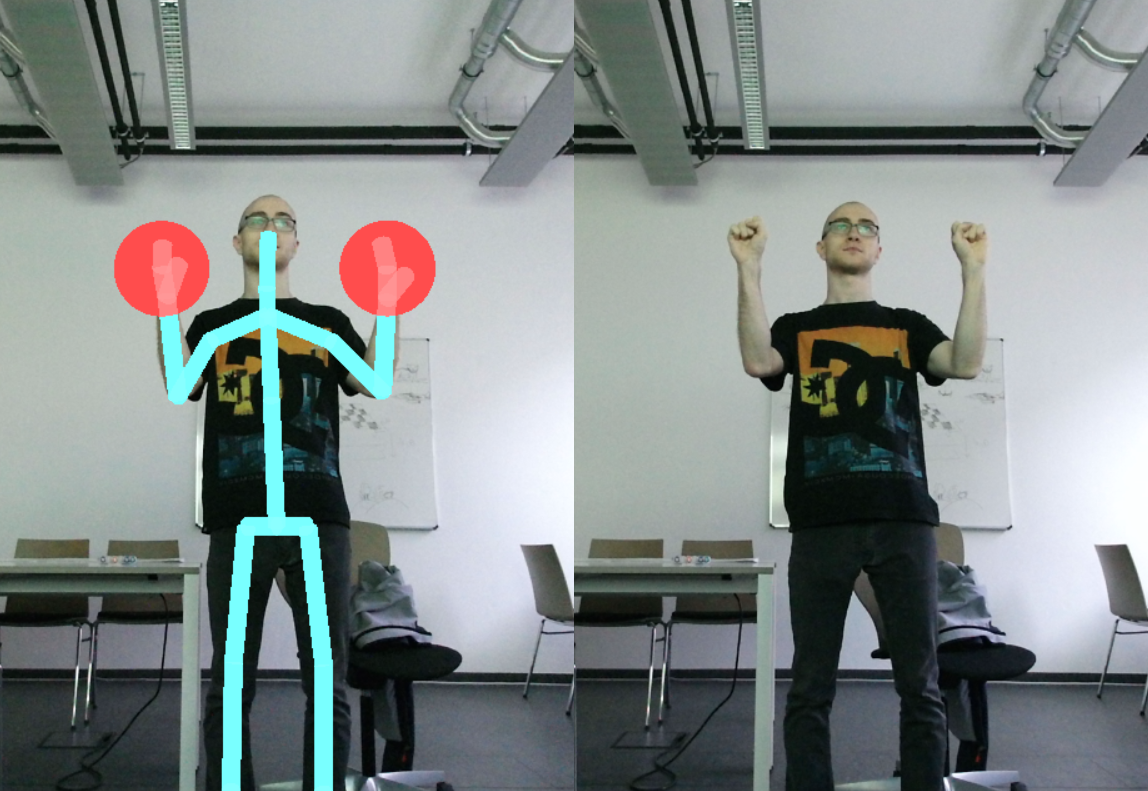
\includegraphics[width=.8\textwidth]{pictures/rotate_.png}
		\caption{Die (Kamera-)Rotations-Geste, mit und ohne eingezeichnetes Skelett und HandStates.}\label{fig:rotateg}
		\end{figure}		
		\par
		\item[GRAB\_GESTURE] (siehe Abb. \ref{fig:grabg})\par
		Zunächst war angedacht, dass die Objektmanipulation dieselben Gesten verwendet wie die Kameramanipulation und die Unterscheidung, was manipuliert wird durch einen globalen Zustand gefällt wird. Bei näherer Betrachtung dieses Ansatzes und ersten Tests dessen fiel auf, dass es so schwierig ist, zwischen Kamera- und Objektmanipulation zu wechseln. Weiterhin schien es während des Testens weniger intuitiv als zuvor angenommen, ein Objekt auf diese Art und Weise zu manipulieren. Es mussten also andere Ansätze gefunden werden.\par 
		In das Problem der Objektmanipulation eingeschlossen ist das Problem des Object-Pickings, d.\,h. die Auswahl des zu manipulierenden Objekts vom Bildschirm. Auch dies wäre mit der oben beschriebenen Methode, die die Gesten der Kameramanipulation verwendet, nur schwierig und umständlich realisierbar gewesen. Wir näherten uns dem Finden eines neuen Weges diesmal auf einem anderen Weg, nämlich nicht über die Manipulation, sondern über das Picking des Objekts. Schnell einigten wir uns auf das Greifen eines Objekts (eine Hand ist erhoben und geschlossen -- dies motiviert auch den Namen \glqq GRAB\grqq-Geste) als intuitivste Möglichkeit dafür. Von der Idee her sollte ein Hin- und Herbewegen dieser \glqq Kontroll-Hand\grqq{} auch das Objekt hin"= und herbewegen. Nachdem dies zufriedenstellend eingebaut war, widmeten wir uns der Objektrotation, was schnell eine fundamentale Schwäche dieser Geste offenbarte: Die Rotation des Objekts sollte der Rotation der geschlossenen Hand folgen, jedoch ist die Erkennung der Rotation einer geschlossenen Hand durch die Kinect viel zu schlecht, um an dieser Stelle sinnvoll Verwendung zu finden.\par 
		Die Ergebnisse wurden direkt sehr gut, als wir dazu übergingen, die GRAB"=Geste durch eine gehobene und offene (!) Hand zu definieren, da die Kinect so -- wie auch naheliegend -- viel besser erkennen kann, wie die Handfläche gekippt bzw. gedreht ist. Intern behielten wir jedoch den semantischen Namen \glqq GRAB\grqq"=Geste bei.
		\begin{figure}[h!]
		\centering
		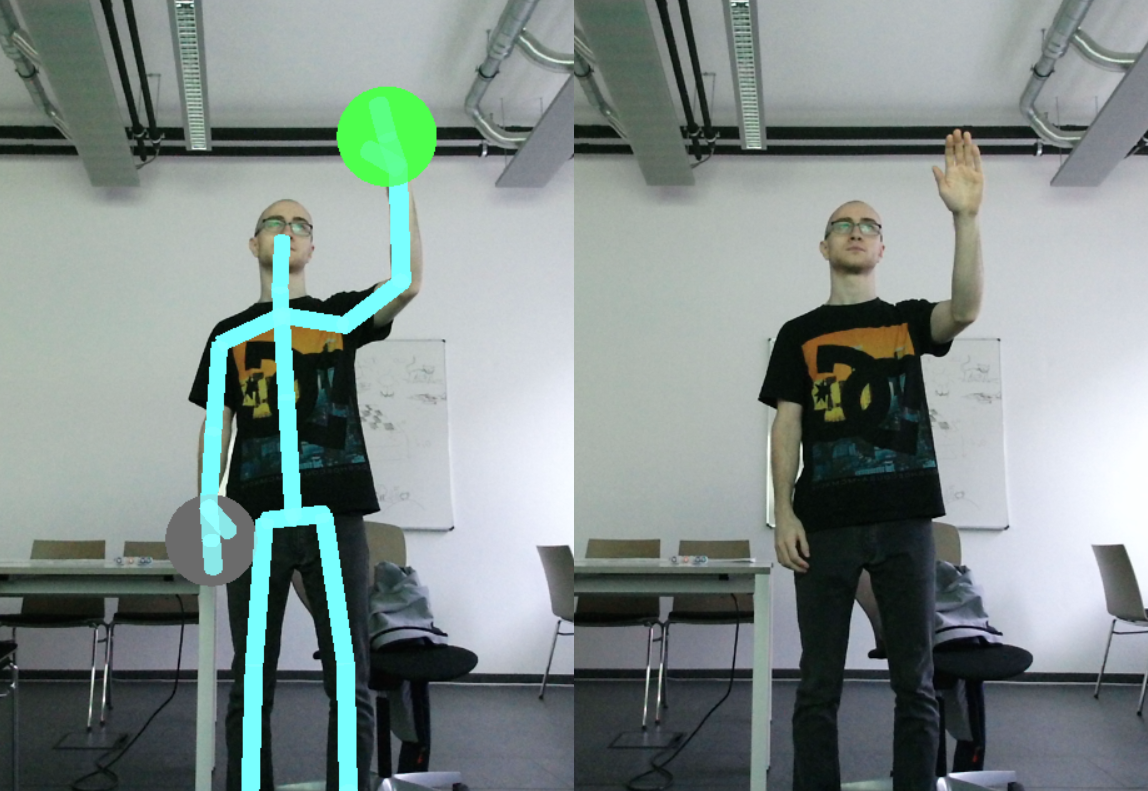
\includegraphics[width=.8\textwidth]{pictures/grab_.png}
		\caption{Die Objektmanipulations-Geste, mit und ohne eingezeichnetes Skelett und HandStates.}\label{fig:grabg}
		\end{figure}
		\par
		\item[FLY\_GESTURE] (siehe Abb. \ref{fig:flyg})\par
		Im Rahmen der Tests mit einem Beispielobjekt wurde schnell deutlich, dass es auch eine einfache Möglichkeit geben sollte, sich über weitere Strecken durch den Raum zu bewegen, ohne dabei ständig zwischen dem Vorführen einer Geste und einem \glqq Nachgreifen\grqq{} wechseln zu müssen. Als sinnvoll erschien hier, dass das Vorführen einer besonderen Geste bewirkt, dass die Kamera losfährt und erst anhält, wenn die Geste nicht mehr präsentiert wird.\par 
		Die FLY"=Geste entspricht dem Ausstrecken beider Arme vor den Körper, sodass sich die Hände mehr oder weniger am selben Punkt im 3D"=Raum befinden. Passiv findet bei dieser Geste im Programm eine Bewegung nach vorne statt. Durch Schwenken der Arme soll der Nutzer dabei die Richtung der Bewegung beeinflussen können, d.\,h. ein Zeigen der Arme nach oben bewirkt, dass die Bewegung immer weiter nach oben gezogen wird, während man mit einem Zeigen nach links oder rechts eine Kurve fliegen kann. Dabei bestimmt der Ausschlag der Arme beim Zeigen (verglichen mit der Ausgangsposition, in der beide Arme genau nach vorne gerichtet sind) die Stärke der Richtungsänderung. Um eine sogenannte Fassrole durchzuführen oder sich in Kurven legen zu können, kann der Nutzer nebenbei seine Schulterpartie in die entsprechende Richtung kippen. Insgesamt ist die Steuerung des Flugmodus in ihrem Funktionsumfang damit ähnlich zu üblichen Steuerungen von Flugzeugen in Actionspielen oder Simulationen.\par 
		Nicht zuletzt daher ist die assoziierte Geste für den Nutzer angenehm und intuitiv und ermöglicht eine im Gegensatz zur Bewegung über Drehen und Schieben einfache Möglichkeit, sich etwa durch ein System von Gängen in einer 3D"=Szene zu bewegen und generell Strecken zurückzulegen, statt Objekte zu betrachten. Ein, wenn auch in der Art der Gesamtanwendung begründetes Problem, ist jedoch, dass das Ausführen dieser Geste durch die nach vorne ausgestreckten Arme schnell anstrengend wird. Für Anwendungen, in denen -- nicht wie in unserem Fall -- der Hauptfokus tatsächlich auf dem Überwinden von längeren Strecken liegt, etwa in einem Rennspiel o.\,Ä., wäre es vermutlich notwendig, diesem Punkt erneut Beachtung zu schenken. Für unsere Aufgabenstellung ist die genannte Gestenvariante jedoch völlig ausreichend und besticht durch Intuition und Immersion.
		\begin{figure}[h!]
		\centering
		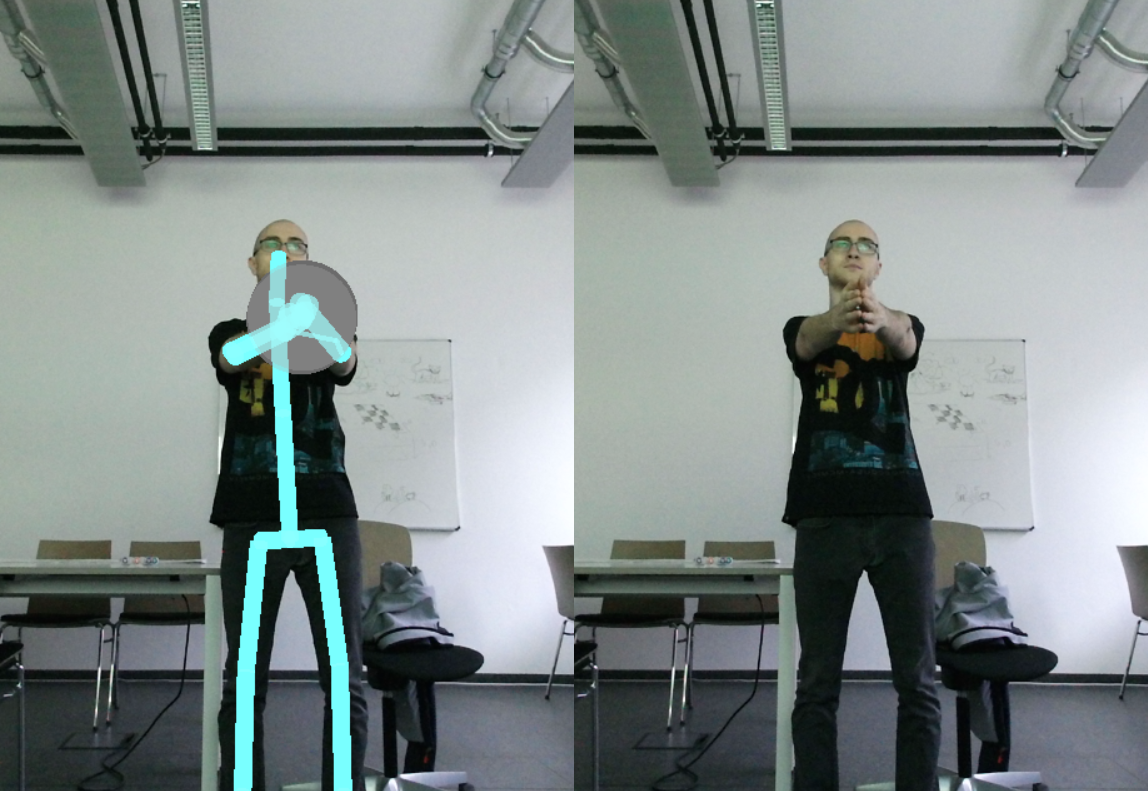
\includegraphics[width=.8\textwidth]{pictures/fly_.png}
		\caption{Die Flug-Geste, mit und ohne eingezeichnetes Skelett und HandStates.}\label{fig:flyg}
		\end{figure}\par		
		\item[UNKNOWN] Dies enthält alles, was als keine der anderen Gesten erkannt wird. Die Kamera und geladene Objekte sollen, solange diese Geste gezeigt wird, stillstehen.\par
		Neben der naheliegenden Motivation, dass der Nutzer die Szene gegebenenfalls auch bei Ruhe betrachten möchte, dient diese \glqq Geste\grqq{} (oder besser \glqq Nicht-Geste\grqq{}) darüber hinaus noch einem anderen Zweck. Sie kann in andere Gesten, wie beispielsweise Translationen, eingebaut werden, um diese aufzubrechen und \glqq nachgreifen\grqq{} zu können. Erst dies gestattet dem Nutzer, während der Bedienung an Ort und Stelle stehen bleiben zu können.
	\end{description}
	Tests mit der Kinect haben ergeben, dass es notwendig ist, bei derartig selbst implementierten Gesten auch eigene Robustheitsmechanismen einzubauen, die die Gestenerkennung gegen Schwankungen der Kinecterkennung (etwa des Status einer Hand) abhärten. Für genauere Informationen hierzu verweisen wir auf Abschnitt \ref{sec:robustheit}.
	\subsection{Zustandsmaschine}
	Das Programm besteht aus zwei Grundmodi der Manipulation: Einerseits der Manipulation der Kamera und andererseits jener des Objekts. Wir können diese beide Modi als zwei Superzustände auffassen, innerhalb derer sich wiederum unterscheidet, auf welche Art und Weise wir manipulieren. Die Zustandsmaschine dient einerseits der Kapselung und Modularisierung der von uns bereitgestellten Funktionen und bildet andererseits die Struktur unserer Manipulationsmodi abstrakt ab.\par 
	Die Zustandsmaschine befindet sich zu jedem Zeitpunkt in einem Zustand. In diesem Zustand findet eine Berechnung der Parameter statt, die unser Programm zurückgibt, die wiederum die Manipulation beschreiben, die ausgeführt werden soll. Dies geschieht durch Auswertung der gesehenen Geste und die Berechnung entscheidender Größen, u.\,U. unter Einbeziehung der Werte vergangener Frames. Schließlich erfolgt basierend auf der präsentierten Geste ein Zustandswechsel am Ende eines Berechnungsschritts. Die Zustandsmaschine ist in Abb. \ref{fig:sm} zu sehen. Im Folgenden erklären wir die Zustände, ihre Semantik und die enthaltenen Berechnungen etwas näher:
	\begin{description}
		\item[IDLE] Dieser Zustand entspricht dem Initialzustand unserer Zustandsmachine. Er ist eine Art Default-Zustand, in dem keine Kamera- und auch keine Objektmanipulation (genauer: keine Berechnung überhaupt) vorgenommen wird. Der Zustand wird betreten, wenn keine der vordefinierten Gesten sicher genug erkannt wurde. Durch Ausführung der entsprechenden Gesten gelangt man zurück in die anderen Zustände.
		\item[CAMERA\_TRANSLATE] Dieser Zustand gehört zur Kameramanipulation. In ihm werden gemäß der oben erklärten Geste die Parameter zur Kamerabewegung bestimmt. Wir berechnen dazu aus den gepufferten Positionswerten von linker und rechter Hand die diskrete Ableitung, die uns ein Maß für die Geschwindigkeit der Bewegung liefert. Ebenso erhält man daraus die Richtung, in die die Hände bewegt wurden. Aus diesen Größen berechnen wir Translationsparameter für die $x$"=, $y$"= und $z$"=Richtungen, die für diesen Zustand unsere \texttt{motionParameters} definieren. %TODO
		\item[CAMERA\_ROTATE] Dieser Zustand gehört ebenfalls zur Kameramanipulation. Analog zu oben wird hier die Rotation vorbereitet. %TODO
		\item[FLY] Dieser Zustand wurde nachträglich eingeführt, als die Notwendigkeit eines Flug-Modus deutlich wurde. Er wird mittels Vorführung der FLY"=Geste betreten und analog zu den anderen Zuständen verlassen. %TODO
	\end{description}
	Zur Verdeutlichung sei darauf hingewiesen, dass von jedem Zustand zu jedem anderen übergegangen werden kann, wobei dieser Übergang lediglich anhand erkannter Gesten erfolgt: Wird eine unserer Gesten erkannt (Details siehe Abschnitt \ref{sec:robustheit}), so wird der zugehörige Zustand betreten. Da unser Programm darauf ausgelegt ist, während des Event-Loops einer Hauptanwendung zu laufen, besteht die Zustandsmaschine ab ihres Starts permanent (bzw. bis zum Ende der Hauptanwendung) und besitzt keinen Finalzustand.\par
	Genaueres zum Aussehen der State-Machine als Datenstruktur ist in Abschnitt \ref{sec:ds} zu finden.
	\begin{figure}[h!]\label{fig:sm}
	\centering
	\usetikzlibrary{positioning}
\resizebox{\linewidth}{!}{
\begin{tikzpicture}

%%IDLE-State
\umlbasicstate[x=0, name=IDLE, fill=white]{IDLE}

%%INIT-State
\umlstateinitial[left=2cm of IDLE.west, name=INIT]
	\umltrans{INIT}{IDLE}

%%Superstate Kamera-Manipulation
\begin{umlstate}[x=0,y=8,name=CAM, fill=black!20]{Kamera-Manipulation}
	%%%%%%%%%%%%%%
	%% Zustände %%
	%%%%%%%%%%%%%%
	%%Zustand Kamerabewegung
	\umlbasicstate[x=0,y=0, name=CAMTRANS, fill=white]{CAMERA\_TRANSLATE}
	%%Zustand Kameradrehung
	\umlbasicstate[x=8,y=0, name=CAMROT, fill=white]{CAMERA\_ROTATE}
	
	%%%%%%%%%%%%%%%%%%
	%% Transitionen %%
	%%%%%%%%%%%%%%%%%%
	\umlHVHtrans[anchor1=20,anchor2=170,arg={ROT...},pos=1.5]{CAMTRANS}{CAMROT}
	\umlHVHtrans[anchor1=-170,anchor2=-20,arg={TRA...},pos=1.5]{CAMROT}{CAMTRANS}
	
	\umltrans[recursive=-120|-170|3cm, recursive direction=bottom to left, arg={TRANSLATE\_GESTURE},pos=1.3]{CAMTRANS}{CAMTRANS}
	\umltrans[recursive=-10|-60|3cm, recursive direction=right to bottom, arg={ROTATE\_GESTURE},pos=2.6]{CAMROT}{CAMROT}
\end{umlstate}


%%Superstate Objekt-Manipulation
\begin{umlstate}[x=8, name=OBJ, fill=black!20]{Objekt-Manipulation}
	%%%%%%%%%%%%%%
	%% Zustände %%
	%%%%%%%%%%%%%%
	%%Zustand Kamerabewegung
	\umlbasicstate[y=0,name=OBJMAN, fill=white]{OBJECT\_MANIPULATE}
	%%%%%%%%%%%%%%%%%%
	%% Transitionen %%
	%%%%%%%%%%%%%%%%%%
	\umltrans[recursive=-40|-140|2cm, recursive direction=bottom to bottom, arg={GRAB\_GESTURE},pos=1.5]{OBJMAN}{OBJMAN}
\end{umlstate}

\umlVHVtrans[arm1=-1cm,anchor1=-60,anchor2=-150,arg={GRAB\_GESTURE},pos=1.4]{IDLE}{OBJMAN}
\umlVHVtrans[arm1=-2cm,anchor1=-30,anchor2=-120,arg={UNKNOWN\_GESTURE},pos=1.5]{OBJMAN}{IDLE}

\umlVHVtrans[arm1=4cm,anchor1=130,anchor2=-45,arg={TRANSLATE\_GESTURE},pos=0.5,name=IDLETOCAM]{IDLE}{CAMTRANS}
\umlVHVtrans[arm2=3.75cm,anchor2=120,anchor1=-40,arg={UNKNOWN\_GESTURE},pos=2.1,name=CAMTOIDLE]{CAMTRANS}{IDLE}
\umlpoint{CAMTOIDLE-2}
\umlVHtrans[anchor1=-150]{CAMROT}{CAMTOIDLE-2}
\umlpoint{IDLETOCAM-1}
\umlHVHtrans[arm1=-2cm,anchor1=170]{OBJMAN}{IDLETOCAM-1}

\umlVHVtrans[arm1=2.5cm,anchor1=55,anchor2=-145,arg={ROTATE\_GESTURE},pos=0.5,name=IDLETOCAM2]{IDLE}{CAMROT}
\umlpoint{IDLETOCAM2-1}
\umlHVHtrans[arm1=-3cm,anchor1=-170]{OBJMAN}{IDLETOCAM2-1}

\umlVHVtrans[anchor1=-140,anchor2=155,arm1=-4cm,arg={GRAB\_GESTURE},pos=0.999,name=CAMTOOBJ]{CAMROT}{OBJMAN}
\umlpoint{CAMTOOBJ-4}
\umlVHVtrans[anchor1=-35,arm1=-1cm]{CAMTRANS}{CAMTOOBJ-4}
%\umltrans[recursive=90|180|5cm,recursive direction=top to left,arg={UNKNOWN\_GESTURE},pos=.5]{IDLE}{OBJMAN}
%\umlVHtrans{IDLE}{OBJMAN}
\end{tikzpicture}
}
	\caption{Die Zustandsmaschine. Der nachträglich eingefügte Zustand FLY ist mit allen anderen Zuständen über die entsprechende Geste verbunden und wird von allen Zuständen durch Präsentieren der FLY-Geste erreicht. Aus Gründen der Übersichtlichkeit wurde auf das Einzeichnen dieser Kanten verzichtet.}
	\end{figure}
		\subsection{Robustheit und Pufferung}\label{sec:robustheit}
	Wie wir vorangegangen festgestellt haben, sind einige der Mechanismen, die wir implementieren wollen anfällig gegenüber qualitativ niedrigwertigen Kinectdaten. Tests mit der Kinect haben folgende kritische Situtationen ergeben:
	\begin{itemize}
		\item \textbf{Gelenke und Skelettbestandteile in der Nähe von Objekten und anderen Personen.} Diese können falsch oder verzerrt erkannt werden. So kann etwa die erkannte Handposition zwischen zwei Kinectframes Raumunterschiede von mehreren Metern aufweisen und zurückspringen. Dies kann auch Körperteile betreffen, die vor oder hinter anderen Körperteilen liegen. Für hinter Körpern oder Objekten versteckte Teile ist klar, dass diese von der Kinect nur geraten werden können. Gliedmaßen, die sich vor Körpern (seltener Gegenständen) befinden können durch die Kinect-Optik zum Teil nicht hinreichend von den weiter hinten befindlichen Körperregionen differenziert weren. Das Problem verschärft sich mit zunehmender optischer und räumlicher Ähnlichkeit (Rückstrahlverhalten im sichtbaren Licht und Infrarotlicht sowie annähernd gleiche Entfernung zur Kamera). Ferner steigt die Ungenauigkeit, je weiter man vom \glqq perfekten Abdeckbereich\grqq{} der Kinect entfernt ist.
		\item \textbf{Status der Hände.} Auch bei durchgängiger Aufrechterhaltung eines Handzustands kann es passieren, dass die Kinect vereinzelt falsche Zuweisungen trifft oder keine Zuweisung möglich ist. Besonders schlecht wird die Erkennung, wenn sich die Hände vor dem Körper befinden. Sind die Hände selbst vollständig oder auch nur teilweise verdeckt, ist selbstverständlich ebenfalls keine sinnvolle Erkennung des Handstatus möglich. Hier liegen weitestgehend dieselben Mechanismen zugrunde, die auch die Probleme von Punkt eins verursachen.  
		\item \textbf{Jitterfehler.} Die Kinectdaten sind verrauscht und weisen bspw. von Frame zu Frame kleine Ungenauigkeiten und Abweichungen der Gelenkpositionen in beliebige Richtungen auf. Diese Fehler nehmen ebenfalls umgekehrt Proportional zur Kinect-Sicherheit zu, d.\,h. treten vermehrt auf, wenn die genaue Position nicht richtig erkannt wird und ein \glqq Rateeinfluss\grqq{} vorhanden ist. Insbesondere ist dies wieder bei Verdeckung (egal in welcher Reihenfolge) mit optischer und räumlicher Nähe der Fall. Dieser Punkt sei jedoch von Fehlern nach Punkt eins insofern abgegrenzt, dass wir uns hier auf ständig auftretende, von ihrer Natur her kleine Fehler beziehen, obwohl Punkt eins natürlich auch bewirken kann, dass die Kinectdaten in beliebige Richtungen \glqq zittern\grqq{}.
		\item \textbf{Phantome.} Mitunter kann es passieren, dass ein ganzes Skelett an einem Gegenstand hängenbleibt. Dies geschieht, wenn eine getrackte Person einen Gegenstand passiert und dabei nicht korrekt erkannt wird -- etwa weil sich die Situation sehr nahe am Rand des Aufnahmebereichs abspielt oder der Gegenstand eine nahezu humanoide Form hat. Sobald die Person wieder richtig erkannt wird, erhält sie ein neues Skelett. Die Skelettdaten dieser Phantome sind dann abgesehen von der Orientierung an menschenähnlichen Merkmalen komplett geraten und variieren über die Zeit sehr stark und willkürlich.
	\end{itemize}
	\begin{figure}
	\centering
	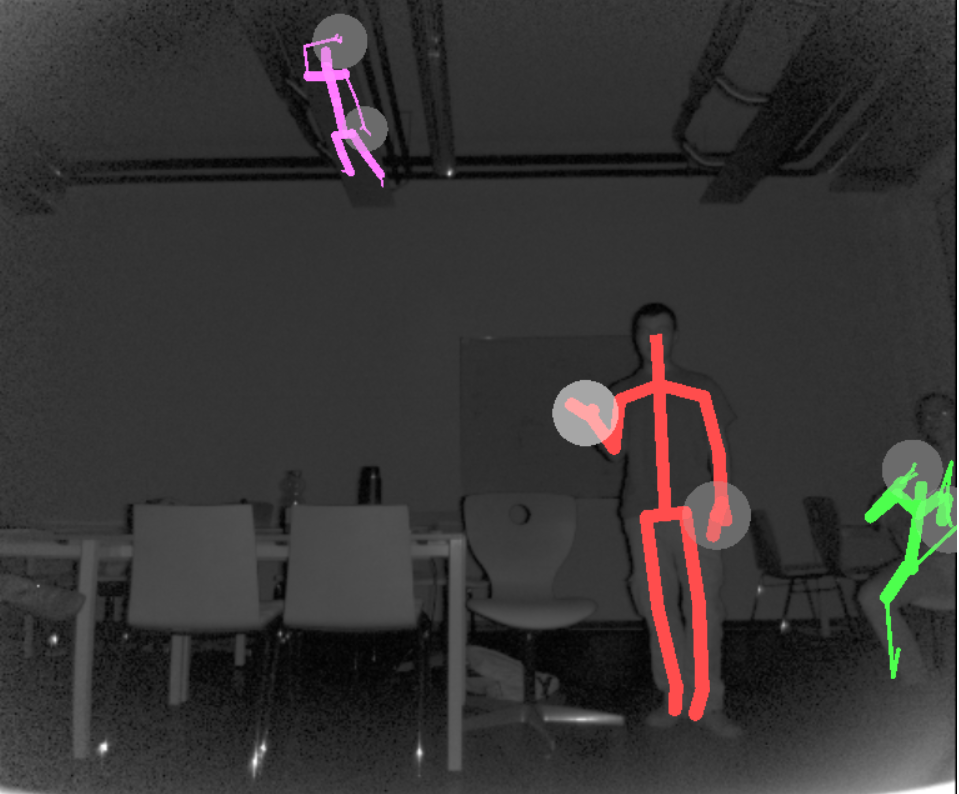
\includegraphics[width=.7\textwidth]{pictures/ninja.png}
	\caption{Infrarotbild der Kinect mit Phantom (oben links entlang der Lampe erkannt). Insbesondere werden Teile des Phantoms von der Kinect mit hoher Konfidenz erkannt (verdeutlicht durch die dicken Linien).\\
	Ferner verzerrtes Skelett am rechten Rand (verursacht durch Verlassen des Aufnahmebereichs).}
	\end{figure}
	Diese Punkte können gravierende Einschränkungen bezüglich der Programmbedienbarkeit mit sich ziehen. Eine fehlerhafte Erkennung von Positionen gemäß des ersten Punktes kann zu einem gänzlichen Verlust der gegenwärtigen Position im virtuellen Raum führen: Im naiven Ansatz wird ein hoher Differenzwert zwischen den die Bewegung (oder Drehung) bestimmenden Handpositionen festgestellt, der die Stärke der Manipulation besimmt und demzufolge auch eine extrem starke Manipulation bewirkt. Bei der Arbeit mit der Objektsteuerung ist ein weiteres Fehlerszenario aufgefallen, welches man als Sonderfall dieses Punktes betrachten kann: Ist die Hand des Nutzers, mit welcher dieser das Objekt bewegt oder dreht, durch die Kinect genau im Profil zu sehen, d.\,h. die Handfläche ist bezüglich der Höhenachse 90 Grad verdreht, so kann die Kinect nicht genau erkennen, in welche Richtung sie verdreht ist (m.\,a.\,W., ob sich der Daumen vorne oder hinten befindet). Solange dies der Fall ist, kann es passieren, dass die Kinect zwischen beiden Möglichkeiten hin- und herspringt, was sich in einer plötzlichen und äußerst starken Drehung wiederspiegelt, der jedoch keinerlei bewusste Nutzereingabe zugrunde liegt.\par 
	Eine fehlerhafte Erkennung nach Punkt drei verursacht durch die vielen willkürlichen kleinen Bewegungen eine als \glqq zittrig\grqq{} wahrgenommene Steuerung der Anwendung: So nimmt ein bewegtes Objekt etwa eine Vielzahl kleiner Bewegungen bzw. Drehungen in verschiedene Richtungen vor, ohne dass der Nutzer eine entsprechende Geste präsentiert hat.\par 
	Das vorübergehende Verlieren (oder Missinterpretieren) des vorgeführten HandStates (Punkt zwei von oben) äußert sich bei der Programmsteuerung dagegen in einem Stottern, d.\,h. dass die ursprünglich fortlaufend präsentierte Geste zu den Zeitpunkten der Fehlerkennung nicht wirkt und daher z.\,B. eine kontinuierlich angedachte Bewegung mehrfach abrupt unterbrochen wird. Siehe Abb. \ref{fig:fehlerk} für eine Illustration.\par 
	Die Erzeugung eines Phantoms ist vor allem dann kritisch, wenn das Phantom aus dem augenblicklichen Master hervorgeht. In diesem Falle übernimmt das Phantom die Programmsteuerung, wodurch einerseits der eigentliche Master die Kontrolle verliert, aber auch andererseits das Programm gänzlich chaotische Bewegungen und Drehungen vornehmen könnte. Letzteres ist wegen der Mechanismen zur Gestenerkennung jedoch unwahrscheinlich, da das Phantomskelett die entsprechenden, relativ strengen Constraints  erfüllen müsste, um den Idle-Modus zu verlassen, nach seiner Erzeugung das Programm aber  sehr schnell in den Idle-Modus bringt.
	\begin{figure}
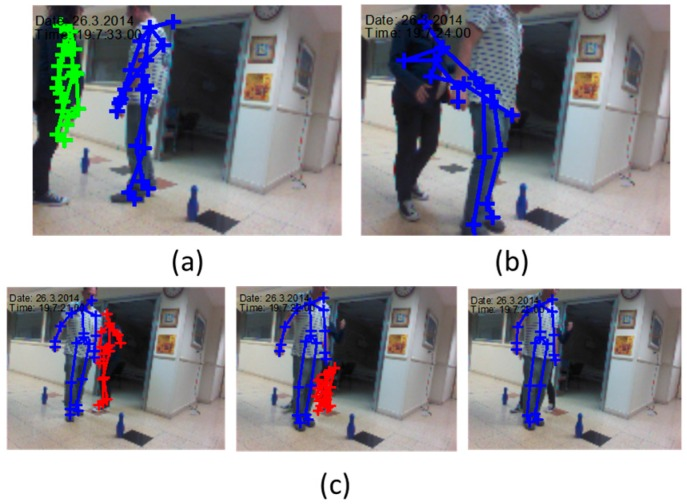
\includegraphics[width=\textwidth]{pictures/sensors-16-01965-g006.jpg}
\caption{Diverse falsch erkannte Skelette.
\begin{enumerate}[label=(\alph*)]
\item degenerierte Skelette
\item verschmolzenes Skelett
\item Skelettverlust durch Verdeckung
\end{enumerate}
Quelle: \cite{bodyprop}}
\label{fig:fehlerk}
\end{figure}
\par
	Diese Probleme üben einen negativen Einfluss auf die Erfahrung aus, die der Nutzer mit der Software macht. Insbesondere Fehler nach dem erstgenannten Schema können dem Nutzer das Erreichen seines Zieles -- etwa des Annavigierens eines Objektes -- unmöglich machen. Die weiteren Punkte werden dagegen einfach als störend empfunden. Die verschiedenen (und auch üblichen) von uns angewendeten Mechanismen, um diese Probleme zu beheben, sind weiter unten erklärt.\par
	Die genannten Schwierigkeiten ergeben sich aus den üblichen Problemen von Sensoren, wobei hier hinzukommt, dass die Kinect (wegen der primären Anwendung, die die Spieleindustrie zum Ziel hatte) über vergleichsweise preiswerte Sensoren verfügt. In diversen Arbeiten, die sich mit ähnlichen Problemstellungen beschäftigen, finden die Grenzen der Kinect nahezu durchgängig Erwähnung und ein wesentlicher Punkt in der Auseinandersetzung mit der Kinect und ihrer Anwendung in unserem und ähnlichen Szenarien widmet sich einer möglichst fehlerarmen Auswertung der qualitativ durchwachsenen Daten. In der Regel wird dabei auf Verzerrungen und schlechte Werte eingegangen, die sich durch den eingeschränkten \glqq Abdeckbereich\grqq{} der Kinect und den Einfluss von Licht ergeben (siehe \cite{bodyprop} und \cite{kinectlight}). Ferner wird darauf hingewiesen, dass das Detektions- und Trackingproblem generell von Beleuchtung, Blickwinkel, Distanz und weiteren Faktoren abhängt (vgl. \cite{thermalsens}). Ferner ist ein gerade für uns wichtiger Punkt die Abhängigkeit der Kinect-Daten von der Pose, was etwa bereits in \cite{biomid} festgestellt wurde. So ist es beispielsweise möglich, durch ungünstiges Verdecken von Körperpartien die durch die Kinect erkannten Gelenkpositionen zu verschieben. Im Test konnten wir so eine Verschiebung des Genicks (gemeint ist der Gelenkpunkt zwischen Schultern und Hals bzw. Kopf) um mehrere Zentimeter reproduzieren, indem die Hände vor dieser Stelle auf und ab bewegt werden. Besonders kritisch ist dies vor allem dann, wenn die Verdeckung nach dem Verschieben aufgehoben wird und der Gelenkpunkt an seine eigentliche Position \glqq zurückschnappt\grqq{}.
	Der ursprüngliche Ansatz, Pufferung und Mittelung, eliminiert die jitterartigen Fehler, mit denen die Kinectdaten häufig belastet sind. Hierzu wird ein Puffer vorher festgelegter Länge verwendet und während des Programmablaufs mit den für den Anwendungszweck wichtigen Daten, hier den Handpositionen des Nutzers gefüllt. Wenn unser Programm schließlich die Rückgabeparameter für die Manipulationen bestimmt, wird dieser Puffer ausgewertet. Wir bilden dabei ein exponentiell gewichtetes Mittel der gepufferten Positionen. Die neuesten Puffereinträge werden am stärksten gewichtet. Dieser Puffer dient dabei noch gleich einem anderen Zweck: Tests haben ergeben, dass das Steuern angenehmer ist, wenn die Übertragung nicht vollständig direkt von den Handpositionen erfolgt. Die Pufferlänge wurde genau so angelegt, dass das dadurch erzeugte Delay dem Nutzer nicht unangenehm auffällt und gleichzeitig die Kontrolle über das Programm per Gestensteuerung wesentlich glatter und angenehmer erfolgen kann.\par 
	Die eben beschriebene Glättung mag zwar kleine Jitterfehler ausmerzen, versagt jedoch bei Kinectdaten, die sehr stark von den eigentlichen Realdaten abweichen. Ein Beispiel für dieses immer wieder auftauchende Problem ist etwa ein weiterer Nutzer der sich im Hintergrund des steuernden Nutzers bewegt. In einem solchen Fall (und ähnlichen Fällen) kann es passieren, dass die Kinect Körperteile dieses zweiten Nutzers falsch interpretiert und dem Steuernden zuordnet. Dadurch können z.\,B. Positionsdaten entstehen, die um mehrere Meter von der Realtität abweichen. Diese Fehler benötigen eine eigene Ausreißerbehandlung: Werte, die eine zu große Abweichung von den zuletzt ermittelten Werten aufweisen (etwa eine Änderung der Handposition um mehrere Meter in aufeinanderfolgenden Frames) und daher unplausibel sind, werden auf eine vordefinierte Maximalabweichung geclippt. Ohne eine solche Behandlung hätten diese Ausreißer dazu führen können, dass der Nutzer seine aktuelle Position in der 3D-Welt ohne sein Zutun mit großer Geschwindigkeit verlässt (falls er sich etwa im Kamerabewegungsmodus befand).\par 
	Mit den gerade besprochenen Methoden haben wir also eine Reihe von Robustheitsmechanismen, was fehlerhafte Kinectdaten hinsichtlich der Position von Joints (Gelenkpunkten) angeht. Dies ist nicht der einzige Aspekt der Anwendung, der solche Sonderbehandlungen verlangt. Wir hatten oben bereits als einen derartigen Punkt die Erkennung der \glqq Hand States\grqq{} genannt. Hier ist insbesondere kritisch, dass eine Fehlerkennung nach dem ursprünglichen Modell, das nur Handzustände zu einem bestimmten Zeitpunkt diskret ausgewertet hat, zu sofortigen Zustandswechseln der Zustandsmaschine führen konnte. Besonders häufig erkennt die Kinect Handzustände in den Fehlersituationen gar nicht (und drückt dies durch \glqq Erkennen\grqq{}) des Zustands \glqq{}Unknown\grqq{} aus), teils -- wenn auch deutlich seltener -- werden jedoch auch die \glqq echten\grqq{} Zustände \glqq offen\grqq{}, \glqq geschlossen\grqq{} und \glqq Lasso\grqq{} falsch zugeordnet.\par 
	Wir wollen ferner Folgendes bemerken: Obwohl die Kinect (auch nicht intern) über keine eigenen Identifikationsmechanismen verfügt (vgl. \cite{bodyprop}), legt die durch das im SDK enthaltene Kinect Studio (siehe \cite{kinectsdk}) nahe, dass wenigstens von der Kinect mitgelieferte Konfidenzwerte für die Güte der Rückgabedaten verfügbar sind. Diese Überlegung drängte sich auf, da schlecht erkannte Gelenke (bzw. eher Gelenkverbindungen) im Studio dünner dargestellt werden, als jene, bei denen die Kinect-Daten gut zu sein scheinen: Dünne Verbindungen treten überwiegend bei Verdeckung und am Sichtfensterrand auf. Es stellte sich jedoch heraus, dass alles, was die Kinect in dieser Hinsicht bereitstellt aus drei Status pro Gelenkpunkt besteht: Jeder Gelenkpunkt ist getrackt (\glqq Tracked\grqq), nicht getrackt (\glqq NotTracked\grqq) und vermutet (\glqq Inferred\grqq). Über den letzten Status ist der Dokumentation (siehe \cite{trackingstate}) nur zu entnehmen, dass das Vertrauen in die Richtigkeit der Daten \glqq sehr gering\grqq{} ist.\par\bigskip
	Abschließend sei noch ein Szenario genannt, gegen das unsere Robustheitsmechanismen keinen hinreichenden Schutz bieten: Das der gezielten Manipulation. Wie bereits bemerkt, sind die Kinectdaten z.\,T. ungenau, etwa bezüglich der Gelenkpositionen. Durch (gegebenenfalls bewusstes) Verdecken oder Unkenntlichmachen von Körperteilen ist es möglich, die von der Kinect erkannten Jointkoordinaten zu verschieben. Dies kann durch den Einsatz von der Hände und der Körperhaltung, aber auch z.\,B. durch weite Kleidung hervorgerufen werden. Wir erklären das Problem an einem Beispiel: In unserer Mastererkennung verwenden wir neben anderen Körpermerkmalen etwa die Torsolänge. Ein Nutzer, der von der Kinect getrackt wird, kann jedoch die an ihm erkannte Torsolänge (genauer den Abstand zwischen den entsprechenden erkannten Gelenkpunkten) verändern, indem er sich beispielsweise streckt und \glqq groß macht\grqq{} (dies verlängert die erkannte Torsolänge) oder aber sich leicht nach vorne beugt (was die erkannte Torsolänge staucht). Dies eröffnet ihm einen Spielraum bezüglich des genannten Merkmals, in dem er die vom eingespeicherten Master bekannte Torsolänge annähern kann. Ähnliches ist für andere Körperteile reproduzierbar, etwa durch leichtes Beugen der Arme oder Anheben und Hängenlassen der Schultern. Eine weitere, aber weniger relevante Möglichkeit ist auch das Ausnutzen von Kinect-Ungenauigkeiten am Rande ihres Aufnahmebereiches, z.\,B. weit weg von der Kamera. Ihre kleinere Relevanz liegt in der Schwierigkeit begründet, \emph{bewusst} diverse Effekte hervorzurufen, da die Randungenauigkeiten aus Anwendersicht willkürlich und ohne Muster sind.\par
	Für Nutzer, die sich ohnehin aufgrund ihrer Körpermerkmale recht ähnlich sind, ist es bei solchen wie eben beschriebenen Manipulation schließlich nicht mehr sicher möglich, eine korrekte Entscheidung zu fällen. Es sei jedoch noch einmal darauf hingewiesen, dass der Beeinflussungsspielraum relativ gering und damit nur für a priori ähnliche Skelette von Belang ist. Ferner ist es augenscheinlich unmöglich, die Manipulation ohne Debugausgaben der genauen Werte bewusst und gezielt durchzuführen.

%
%
\clearpage
\section{Bemerkungen zum Quellcode}
In diesem Abschnitt wollen wir wesentliche Stellen bzw. Strukturen des Programmcodes etwas technischer erläutern. Wir gehen dazu auf die verwendeten Datenstrukturen, Variablen und Funktionen ein und erläutern grob ihr Zusammenspiel. Schließlich wird in diesem Abschnitt auch auf das Einbinden unseres Programmes zur Verwendung in fremder Software eingegangen.
		\subsection{Wichtige Datenstrukturen, Variablen und Funktionen}
		\subsection{Details zum Zusammenspiel}
		\subsection{Einbinden}
%
%
\section{Schlussbemerkungen}
%TODO verwendete Werkzeuge

\newpage
\printbibliography
\end{document}